
\documentclass[12pt]{amsart}
\usepackage{geometry} % see geometry.pdf on how to lay out the page. There's lots.
\linespread{1.5}
\usepackage{graphicx}
\geometry{a4paper} % or letter or a5paper or ... etc
% \geometry{landscape} % rotated page geometry

% See the ``Article customise'' template for come common customisations

\title{Term Paper - CS350}
\author{Russell Miller and Ben Carr}
\date{\today} % delete this line to display the current date

%%% BEGIN DOCUMENT
\begin{document}

\maketitle
%\tableofcontents

\section*{Introduction}
%\subsection{}

This project is an assessment of several sorting algorithms. We chose to implement four sorting algorithms: 
\begin{itemize}
\item Bubble, average  $O(n^2)$, worst-case $O(n^2)$
\item Insertion, average $O(n^2)$, worst-case $O(n^2)$
\item Quick, average $O(n$ lg $n)$ worst-case $O(n^2)$
\item Merge, average and worst-case $O(n$ lg $n)$
\end{itemize}
These four algorithms were implemented and tested in two languages: C++ and Java. We had initially planned on including Python and Haskell, but due to time constraints and the limitations of Python, we were only able to collect significant data and run analysis on our Java and C++ algorithms. Each program tested 100 completely random unsorted lists of integers, each of size $n = $ \{10, 50, 100, 500, 1000, 5000, 10000, 50000, 100000\}. This paper will discuss our findings, assess our results and communicate to the reader our understanding of how complexity theory comes up in practice. We found that quicksort ran exceptionally fast on these random lists, so additional data (lists size "n" up to 10,000,000 for Java and 100,000,000 for C++) was run on quicksort.\\
\section*{Background}

We split up the main algorithms we would need to write so that each of us would be
writing them in two languages. Russell worked in Java and Python while Ben worked in Haskell and C++. Russell has
written a lot of small Python programs, and a few medium-scale ones. Java was a
major refresher for him, as it has been a while. Ben was fairly new to Haskell and hadn't used C++ much since his freshman year of college, so Russell was helpful when he got stuck. Writing the algorithms themselves took very little time, especially in Python and Haskell. The language is so straight-forward that if you know what you want to do you can have something working in very little time. Later 
in this paper, we'll discuss one of its weak points. We also used Python to 
generate our lists. 

% generating the lists
We decided that it would be good to have a consistent set of lists that are 
randomly generated to use across all of the sorting algorithms and all of the 
languages. The reason behind this was our plan of comparing the implementations across languages, that is, if we wanted to compare one language to another, it would be unfair to compare their performance if they were operating on different data. There were many struggles when we were developing this list generator.
It took several tries to figure out how to build up the right amount of data in 
memory before writing it to a file, because we did not want to spend extra time 
doing more File I/O than necessary. 

At first we started with a very simple program that when given an argument, would
create 1000 new files, each containing a list of the size specified in its 
argument. This worked fine for the first few sizes, so we ran the script in 
separate shells, with different inputs, to get all of our lists ready. However,
the system ran out of memory before it could finish.

Next we decided to write each list to a file, one by one, rather than storing all 
of the information in memory and attempting to write all of the files at the end. 
This worked, but it took quite a considerable amount of time. This is the method we used; it was slow but got the work done.

% struggles with java
One of the biggest struggles we faced while working with Java was determining how 
to store the lists/arrays. At first we just wanted to have an array as a private 
field. We then discovered that most of the algorithms we were working with sorted 
in place, meaning they would change the values in the array. This wouldn't work 
for a class that has four different sort algorithms going in sequence and
accessing the same array, and unfortunately we did not abstract the sorting out 
of the primary class. Rather, we used four arrays, one dedicated to each 
algorithm.

The next tricky thing was figuring out how to run the stopwatch on the 
algorithms while they sort the lists. The way the Java program was laid out, we were able to place the stopwatch calls right next to the sort method calls, and we used public methods to retrieve the times from the private fields they were stored in. We also had trouble with timing our C++ algorithms. Initially we tried using the C++ function \texttt{clock()} from the library \texttt{sys/time.h} which gives clock cycles per second. We wanted it in seconds so ended up trying \texttt{gettimeofday()}, but that function returns seconds (or the nanoseconds AFTER the decimal) so that was a total mess to work with. We ended up using \texttt{clock()} and some simple arithmetic to get the time format to be exactly how we wanted:
\linespread{1}
\begin{verbatim}
// source: http://www.physicsforums.com/showthread.php?t=224989
double diffclock(clock_t t1, clock_t t2)
{
  double diffticks = t2 - t1;
  double diff = diffticks / (double)CLOCKS_PER_SEC;
  return diff;
}
\end{verbatim}
\linespread{1.5}
The final struggle while working in Java, which carried over to implementing it
in C++ as well, was the merge sort. The way we understood the merge sort algorithm
was that it split the list into two smaller lists and recursed down to those. Then
the merge action put the smaller lists back together. Algorithms exist to do this in
place with an array, but the easier implementation was to try the Java \texttt{List} class.
In attempting to learn to use it, we also discovered the magic of the \texttt{ArrayList} class. Basically, it
allows you to do list operations such as \texttt{cons} (Java calls it \texttt{add}), and there is also
a \texttt{get} function that allows you to refer to a specific index. Both of these
operations came in handy. C++ has lists in its standard library, and though it
did not have the get method, it was not difficult to make the translation from
the Java code to the C++ code.

% struggles with list sizes
Once we verified that all of the sorts were in fact sorting, adjusted the output
that would be written to the CSV file, tested the stopwatch, and did a dry-run
on a small set of lists, it was time to ship it. The program ran for two days
and still had not finished. At this point we became very worried, so we tried
timing a single list of size 100,000. In java it only took about 30 seconds, but
in C++ it took 3 minutes. We decided this could be our new size limit, and not
go all the way to one million.

\section*{Findings and Analysis}
Our Java program ran in about 2 hours, and C++ took approximately 3 hours on list sizes $n = $ \{10, 50, 100, 500, 1000, 5000, 10000, 50000, 100000\}. for each $n$, each algorithm ran on 100 lists (the total number of lists the program sorted was $100 * |n| = 900)$. The average time for each algorithm (in seconds) was recorded and can be found in Table 1. We wanted to see how consistent the algorithms were behaving, figures 2-5 shows each trials execution time, (for each algorithm). Finally we wanted to see a comparison of the algorithms against each other, Figure 6 is a graph of the averages as we approach our maximum $n$, using a trend line with regression type "power" for bubble, insertion and merge sort and logarithmic for quick sort. Quicksort ran incredibly fast, so we decided to run it on larger lists (up to n = 10,000,000). Table 2 shows this graph against $n$ log $n$
\\ \\ \\
\begin{table}\footnotesize
\begin{center}
\begin{tabular}{ r | l l l l  }

List Size	&	Quick	&	Bubble	&	Insertion	&	Merge\\ \hline
10			&	0		&	0		&	0			&	0\\
50			&	0		&	0		&	0			&	0\\
100			&	0		&	0		&	0			&	0\\
500			&	0		&	0		&	0			&	0\\
1000			&	0		&	0		&	0			&	0\\
5000			&	0		&	0.05		&	0			&	0.01\\
10000		&	0		&	0.19		&	0.01			&	0.03\\
50000		&	0		&	4.84		&	0.37			&	0.72\\
100000		&	0.01		&	19.4		&	1.51			&	3.03\\

\end{tabular}
\end{center}
\caption{Java average run times (in seconds) of unordered lists.}
\end{table}
\begin{figure}[h]
  \centering
    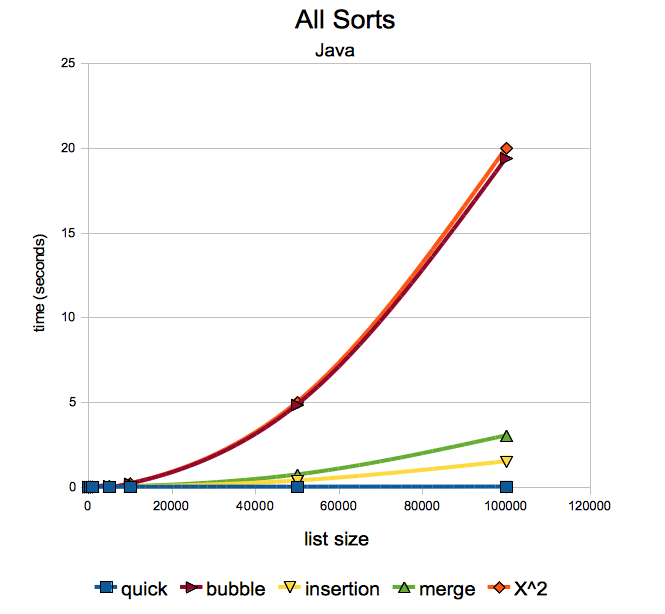
\includegraphics[width=0.9\textwidth]{JAllSorts.png}
  \caption{Behavior of sorts against each other}
\end{figure}

\begin{figure}[h]
  \centering
    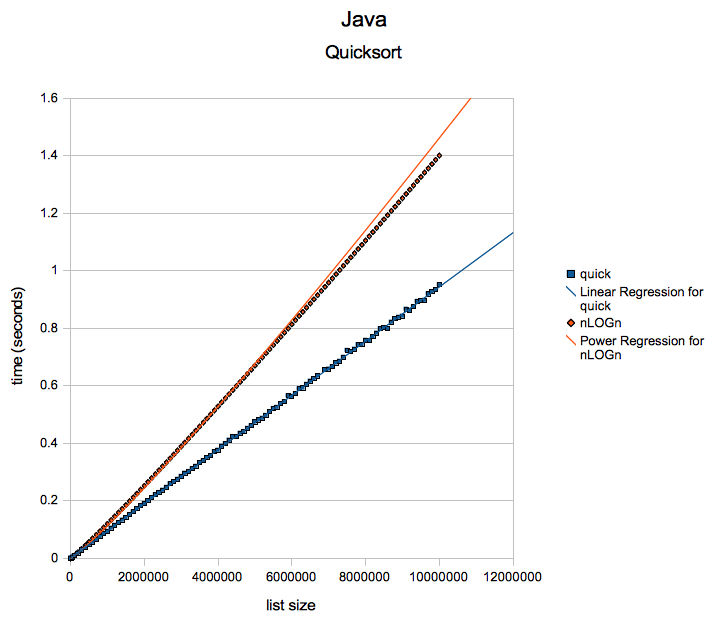
\includegraphics[width=1.0\textwidth]{JHardcoreQS.png}
  \caption{Behavior of quick sort for $n$ up to 10,000,000}
\end{figure}




\section*{Understanding Algorithms}

% understanding algorithms
While putting these sorting algorithms into our programs, one thing that helped
us understand them was to go through them, line by line, with an example on a
dry erase board. In addition, we made sure to test them all and verify that they
were doing their job. The first sort we studied was the Quicksort. It turns out
it is a relatively simple algorithm. When looking at an array of numbers, you
simply pick a value that is present in the array - the pivot - and divide the 
rest of the array based on whether the values are less than or greater than the 
pivot. It's recursive so you then apply this to those two new arrays.

The Quicksort is a strange beast. When compared with the complexity of other
sorting algorithms it doesn't seem to be so great because of the worst case $O(n^2)$ time that it can take. However, it is extremely unlikely for that case to take place. Its performance is also very good on lists that are not "nearly-sorted" which was the type of data we were feeding it.  The behavior of Quicksort for smaller n seems to be much faster than that of the algorithms which do not have as high of a worst-case condition. The
trickiest part is getting a good pivot value. By getting a lucky pivot value the
divide portion of this divide-and-conquer algorithm is more effective. The
reason $O(n^2)$ is possible is that the recursion only stops when the list being
sorted has been reduced to size one. So if every pivot value is the worst
possible pivot value, every divide will result in an empty list, and an n-1
sized list. Figure 1 is a hand-drawn example of Quicksort in action.
\begin{figure}[h]
  \centering
    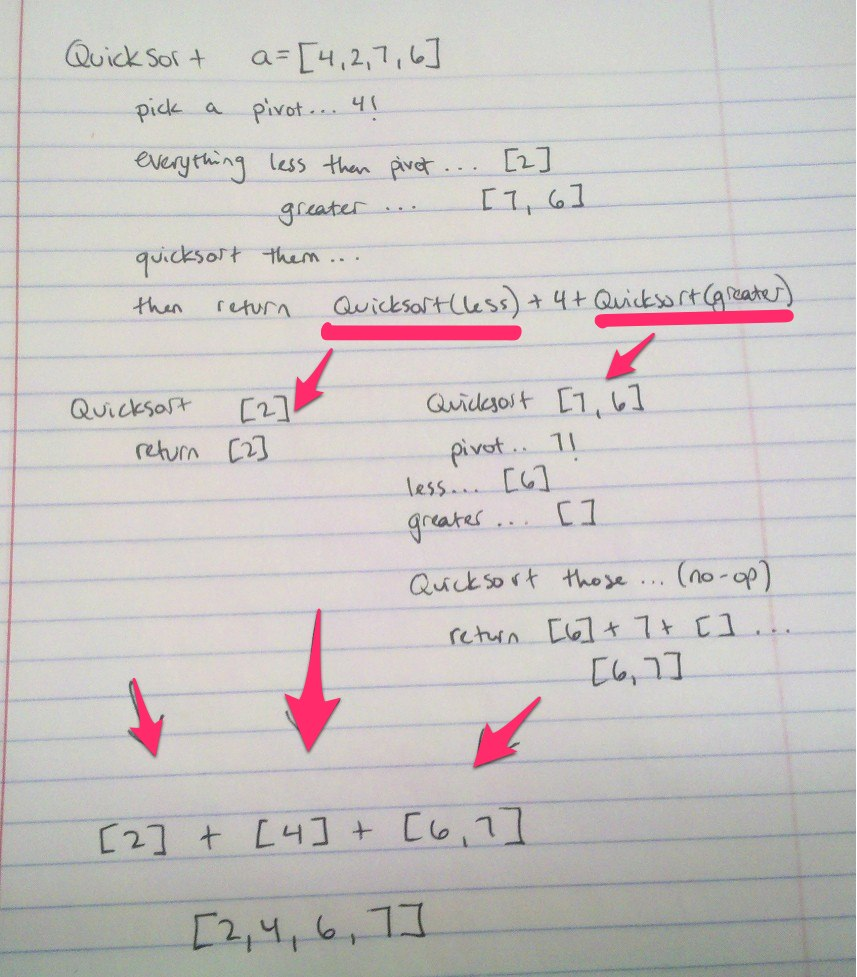
\includegraphics[width=.7\textwidth]{quicksort-drawing.jpg}
  \caption{Walkthrough of quicksort}
\end{figure}

The easiest algorithm to implement was bubble sort

% testing
In order to verify that our algorithms were sound, we implemented a good deal of
testing. The test set was usually the full 100 lists of a specific size, and in
order to verify that the list in question is actually sorted afterwards, we did
a few different things, depending on the language we were working with. Python
has a built in function called sort, so we simply checked that the list we
sorted was the same as the one Python sorted. In Java there was also a built-in
sort function call. In C++ we iterated through the array, making sure that every
value was less than its successor.
\end{document}

